\documentclass{rpt}

\title{Weekly Report}
\author{}
\date{\today}

\begin{document}

\maketitle

\section{Targets}

\subsection{Urgent}
\begin{itemize}
    \item
        Change PI don't care set: simplify CNF by logic synthesis or special input pattern.
    \item
        Change PI care set: use different random seed.
    \item
        Change window don't care set.
\end{itemize}

\subsection{Important}
\begin{itemize}
    \item
        Randomly selecting a node,
        compute its care set,
        change its care set,
        synthesize the local circuit,
        evaluate its area and error rate,
        accept it with a certain probability.
    \item How DC affects BDD\@.
        \begin{color}{red}
            Change simplification method (mfs$\rightarrow$bdd).
        \end{color}
    \item Induce DC with PLA files
    \item Use model counting to compute error rate, i.e., how many assignments satisfying a SAT problem.
    \item Use approximate confidence interval / hypothesis testing of Bernoulli experiments to evaluate the accuracy of error rate.
    \item Trade off the accuracy of batch error estimation for speed
        (even directly use Su's equation to update Boolean difference),
        perhaps use hypothesis testing to evaluate the accuracy.
    \item Combine the simulation of circuits with the simulation of Monte Carlo Tree Search.
        In other words,
        in one loop of Monte Carlo Tree Search,
        merge logic simulation and playout (only simulate circuit once and playout once).
    \item Represent circuit with AIG because of more potential LAC candidates.
        For each round, select one or more input wires and replace them with constant 0 or 1.
        Consider how to combine Wu's method (choose a subset of input wires and substitute).
    \item Accelerate Approximate Logic Synthesis Ordered by Monte Carlo Tree Search:
        reuse the result of batch error estimation in playout.
    \item
        Use UCB1's bound to guide the simulation time.
        Find relationship of different bounds.
\end{itemize}

\subsection{Worth Trying}
\begin{itemize}
    \item Enhance default policy with greedy approach or field domain knowledge.
    \item In expansion process of MCTS, expand more than one layers.
    \item Tune parameters in MCTS\@.
    \item Perform greedy flow on leaves of the final Monte Carlo Search Tree.
    \item Combine beam search and MCTS\@.
    \item
        \begin{color}{red}
        Influence of network representation on synthesis.
        Why does mfs use local AIG function to represent the circuit,
        is it more fittable to LUT mapping?
        \end{color}
\end{itemize}

\subsection{Potential Topics}
\begin{itemize}
    \item Relationship between power simulation and logic simulation.
    \item Combine Binarized Neural Network with approximate computing.
    \item Relationship between Boolean network and Bayesian Network.
    \item Approximate TMR\@.
\end{itemize}

\section{Progress}

\subsection{Issues of Last Meeting}

\subsubsection*{How to synthesize using external don't-cares (EXDCs)}

Alan said that it was possible to use EXDCs in ABC but it was rather complicated.
He recommended me to refer to the SIS script ``full\_simplify'' to handle EXDCs.

\subsection{Issues of This Week}

\subsubsection*{Fixed the bug of logic simulation on AIG network}
Since it is too detailed and not very relevant to the project,
I do not expand here.

\subsubsection*{Set the approximate care set on windows in a circuit}
For a node $f$,
I extract its window $W$.
The ``roots'' of the window are the nodes 2 levels away from $f$ in $f$'s transitive fanouts.
The inputs of the window are the nodes $l$ levels away from $f$ in all the ``roots'' transitive fanins.
However,
the divisors are also the nodes in the transitive fanins of all the ``roots''.

The logic simulation process generates $M$ assignments for the inputs of the window $W$.
Assuming that those $M$ assigments are the approximate care set of the window.
Let $h$ be the corresponding expression of the $M$ assignments.
For example,
if there are 3 assignments for a 3-input window,
010, 100, 111,
then $h=\bar xy \bar z + x \bar y \bar z + xyz$.

The SAT solver is built like the following figure:

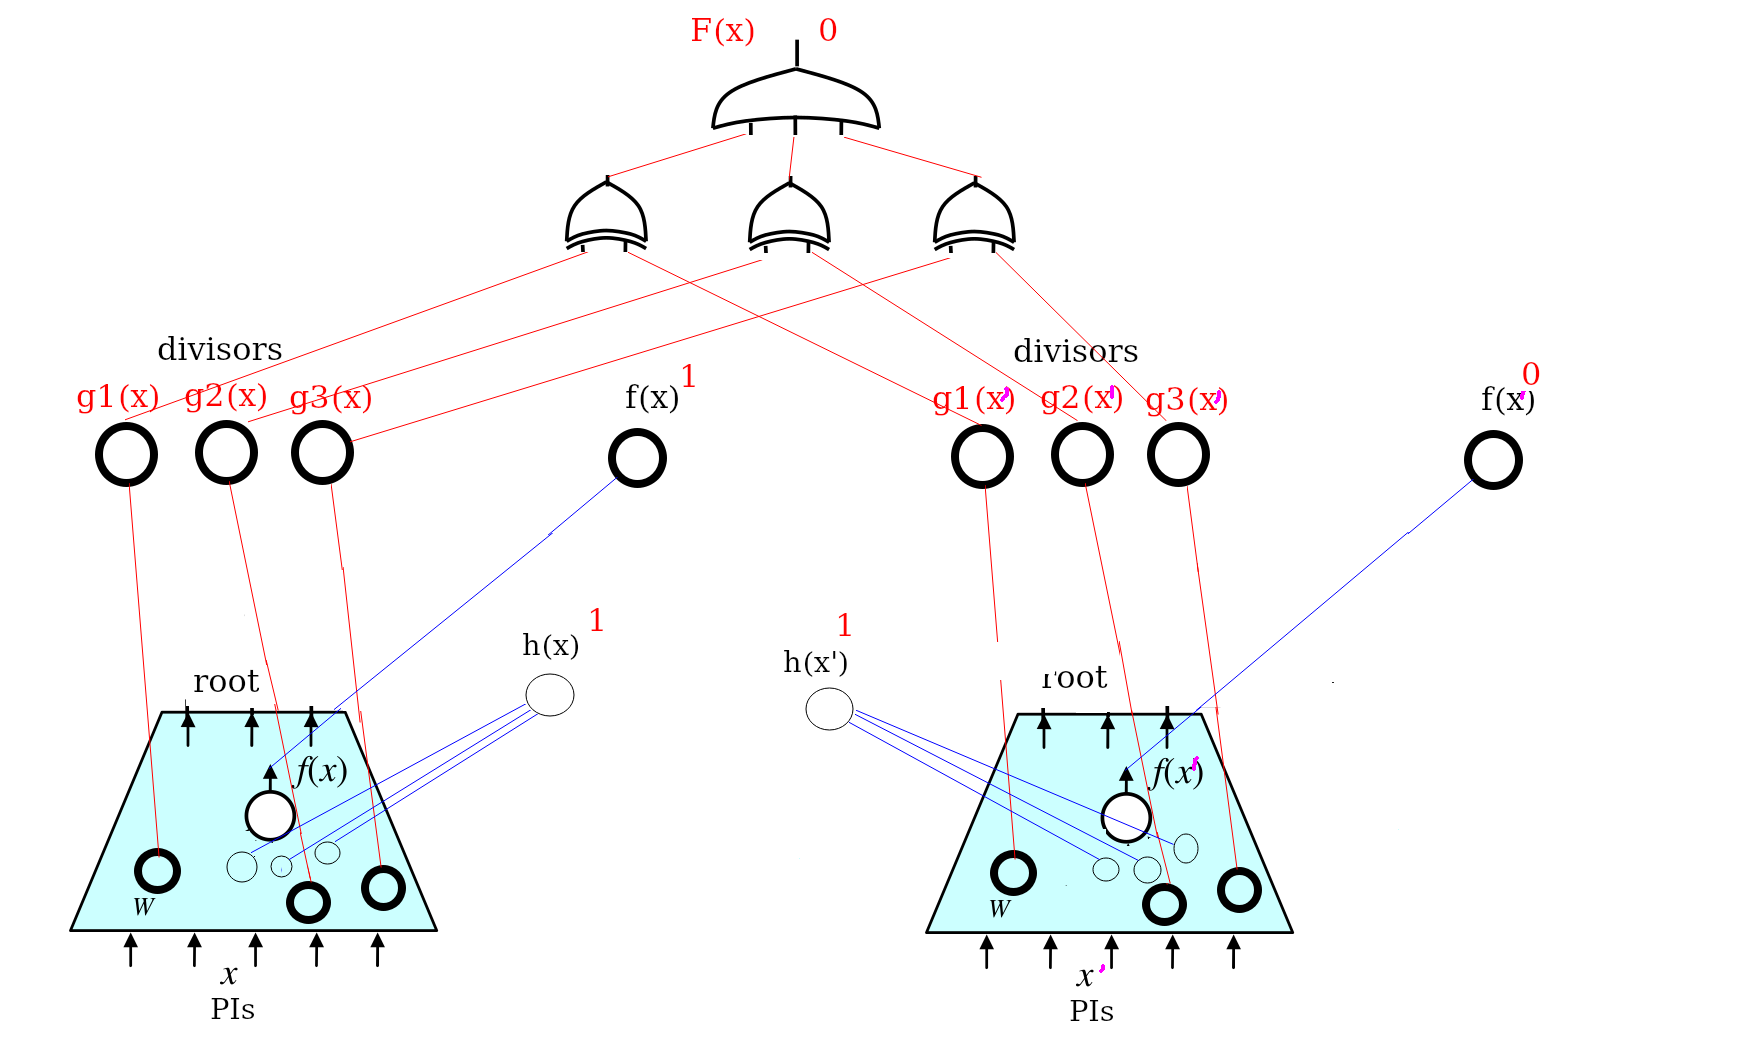
\includegraphics[width=7.0in]{./sat.png}

For $M=10240$, I test the result under different $l$ on c880.
Wu+Su's method can generate an area of 504 under 0.05 error rate.

\begin{tabular}{ccc}
    \hline
    $l$ & final area & error rate \\
    \hline
    1 & 539 & 0.110156 \\
    \hline
    2 & 530 & 0.14248 \\
    \hline
    3 & 517 & 0.150195 \\
    \hline
    4 & 509 & 0.152246\\
    \hline
    5 & 508 & 0.170996\\
    \hline
\end{tabular}

However,
for a fixed $l$,
the result does not change with $M$.
For example,
when $l=3$,

\begin{tabular}{ccc}
    \hline
    $M$ & final area & error rate \\
    \hline
    64 & 517 & 0.150195 \\
    \hline
    1024 & 517 & 0.150195 \\
    \hline
    10240 & 517 & 0.150195 \\
    \hline
\end{tabular}


\end{document}
